% This template is adapted from the CS224N Spring 2024 Project Milestone Template 
% https://web.stanford.edu/class/archive/cs/cs224n/cs224n.1246/project/project-milestone-instructions-spr2024.pdf

\documentclass{article}

\usepackage[final]{neurips_2019}
\setcitestyle{numbers}  % Force numerical citations

\usepackage[utf8]{inputenc}
\usepackage[T1]{fontenc}
\usepackage{hyperref}
\usepackage{url}
\usepackage{booktabs}
\usepackage{amsfonts}
\usepackage{amsmath}
\usepackage{nicefrac}
\usepackage{microtype}
\usepackage{graphicx}
\usepackage{xcolor}
\usepackage{lipsum}
\usepackage{booktabs}
\usepackage{multirow}
\usepackage{xurl}

\newcommand{\note}[1]{\textcolor{blue}{{#1}}}

\title{
  Weekly Report 1 \\
  \vspace{1em}
  \small{\normalfont \today} 
}

\iffalse
\author{
  Ruining Luo \\
  School of Computing and Data Science \\
  The University of Hong Kong\\
  \texttt{ning.l.rn@connect.hku.hk} \\
}
\fi


\begin{document}

\maketitle

\begin{abstract}
This report documents my process of familiarizing myself with the RAG-Anything project through empirical evaluation.
I implemented an LLM-as-a-judge framework to assess the system's performance. 
Initial experiments with LLM-generated QA-pairs from a single PDF, which revealed a need for larger-scale testing. 
Consequently, I evaluated the system on 230 QA items across text, table, figure, and multimodal types from the MMDocIR benchmark\footnote{\url{https://huggingface.co/datasets/MMDocIR/MMDocIR_Evaluation_Dataset}}, 
The results demonstrates the model's relative strength in textual tasks and potential challenges in complex multimodal reasoning, also revealing a need for new evaluation methods for multimodal RAG systems. 
This work serves as a foundation for understanding the project and guiding future improvements.

\end{abstract}

\section{Experiments I}

  \subsection{Evaluation Method}
  I first attempted to evaluate the model with LLM-generated QA-pairs on a single PDF file (the original LightRAG paper).

  I modified \verb|process_with_rag()| to extract text content and multimodal items,
  format context into a QA-pair generation prompt,
  and call the \verb|llm_model_func()| and \verb|vision_model_func()| from the original code to generate a QA-pair for each text-chunk or multimodal item.

  The questions are scored by LLM from 1 to 5 in three dimensions, namely groundness, relevance and stand-alone.
  The QA-pairs with low-scoring questions are removed.

  Then, RAG-Anything is queried with the questions and has the responses collected.
  The responses and the QA-pair are formatted into an evaluation prompt, utilizing another model to score the RAG response from 1 to 5.\footnote{Evaluation script: \url{https://github.com/rnluo/RAG-Anything/blob/main/examples/evaluation_on_single_file.py}}

  The prompts in this section are adapted from Hugging Face\footnote{\url{https://huggingface.co/learn/cookbook/en/rag_evaluation}}.

  \subsection{Results}
    Table \ref{tab:results1} shows the performance of RAG-Anything on four types of QA-pairs.
    The "Threshold" in the table refers to the question quality threshold.
    For instance, when Threshold $=2$, questions scored below 2 in any of the three dimensions are removed.
    When Threshold $=1$, no questions are removed.

    \begin{table}[ht]
        \centering
        \begin{tabular}{l|cc|cc}
        \toprule
        & \multicolumn{2}{c|}{Threshold $= 1$} & \multicolumn{2}{c}{Threshold $= 2$} \\
        Type   & Number of QA-pairs & Avg. Score & Number of QA-pairs & Avg. Score\\
        \midrule
            Text & 65 & 4.28 & 18 & \textbf{4.39}\\
            Table  & 6 & 4.00 & 0 & N/A\\
            Image & 6 & 3.83 & 0 & N/A\\
            Equation & 2 & 3.00 & 1 & \textbf{5.00}\\
        \bottomrule
        \end{tabular}
        \vspace{12pt}
        \caption{Average LLM-judged score of RAG-Anything on four types of LLM-generated multimodal QA-pairs with two question quality thresholds.}
        \label{tab:results1}
    \end{table}

    The results indicate that RAG-Anything may score higher with better QA-pairs.
    However, the number of multimodal questions from a single file is too small to be statistically meaningful.
    Even a minimal increase in the question quality threshold filters out most questions.
    This indicates that it is difficult to generate high-quality QA-pairs and that there is a need to evaluate the model on larger, pre-reviewed datasets.

\section{Experiments II}
  \subsection{Evaluation Method}
  I utilized a subset of the evaluation dataset from MMDocIR\cite{dong2025mmdocirbenchmarkingmultimodalretrieval}, a benchmark for multimodal retrieval.
  The dataset consists of document page screenshots annotated with questions, answers, modality type of the question, and bounding box coordinates of ground truth evidence on pages, etc.
  
  I extracted the first 100 "Pure-text (Plain-text)" questions, 100 "Chart"/"Table"/"Figure" questions, and 30 "multimodal-t"/"multimodal-f" questions.
  For text questions, I save the provided OCR text into temporary files.
  For multimodal questions, I crop relavant screenshots with provided bounding box coordinates and save them as temporary files.
  The temporary files are added into the knowledge base of RAG-Anything, which is queried by corresponding questions.
  The RAG-responses are scored from 1 to 5 with the same evaluation prompt in section 1.
  \footnote{Evaluation script: \url{https://github.com/rnluo/RAG-Anything/blob/main/examples/evaluation_on_dataset.py}}

  Since the QA items are based on independent contexts, RAG-Anything must re-initialize and rebuild the knowledge base for every question, which is computationally expensive and time-consuming.
  This reveals the need for a specially curated dataset in the form of a single, long, multimodal-item-rich document with QA-pairs.

  \subsection{Results}

  Table \ref{tab:results2} shows the performance of RAG-Anything on various types of QA items.

  \begin{table}[ht]
        \centering
        \label{tab:results2}
        \begin{tabular}{l|cc}
        \toprule
          Type in original dataset& Number of QA items & Avg. Score\\
          \midrule
            "Pure-text (Plain-text)" & 100 & 3.33\\
            "Chart" &     33  & 2.42\\
            "Table" &  26 & 3.08\\
            "Figure" &   41 & 2.17\\
            "multimodal-t" &  25 &  2.92 \\
            "multimodal-f" &   5 & 2.20 \\
        \bottomrule
        \end{tabular}
        \vspace{12pt}
        \caption{Average LLM-judged score of RAG-Anything on various types of QA items from the MMDocIR\_Evaluation\_Dataset.}
    \end{table}

  \paragraph{Pure-text questions}
  The score of 3.33 is lower than the previous results with LLM-generated QA-pairs.
  This may result from a discrepancy between the model and the dataset,
  since RAG-Anything returns long and comprehensive responses and the factual answers in the dataset are much more concise.
  It reveals a need for datasets specially constructed for RAG systems.

  \paragraph{Multimodal questions}
  The model scores 3.08 in "Table" questions, significantly higher than in "Chart" and "Figure" questions.
  This may indicate that the model benefits from the provided table processor.

  There is another reason why the model performs worse on multimodal questions than on pure-text questions,
  illustrated in Table \ref{tab:case}.
  The two cases both involve subtracting two figures to obtain the answer.
  While the model succeeds with clear reasoning in the pure-text case, it fails to comprehend the task in the multimodal case, even though the figures are correctly extracted.
  This may indicate that the model can be improved in complex multimodal reasoning,
  especially in the effective comprehension of short texts in multimodal items. 

  \begin{table}[t]
    \centering
    \caption{Case Study: One successful case with text and one failed case with multimodal context.}
    \vspace{-0.08in}
    \label{tab:case}
    \resizebox{\textwidth}{!}{
    \begin{tabular}{|l|p{15cm}|}
    \hline
    \textbf{Type} & "Pure-text (Plain-text)"\\
    \hline
    \textbf{Context} & \textit{[OCR text\dots]}\\
    \hline
    \textbf{Question} & What was the value of absolute percentage shortfall in India's GDP growth from 2002 to 2003 compared to the forecast?\\
    \hline
    \textbf{Answer} & 2.4\%\\
    \hline
    \textbf{RAG-Anything} & 
    The absolute percentage shortfall in India's GDP growth from 2002 to 2003 compared to the forecast can be calculated as follows:\newline
    - Forecast GDP growth: 6.7\%\newline
    - Actual GDP growth: 4.3\%\newline
    The absolute percentage shortfall is calculated as:\newline
    \[ 
    \text{Shortfall} = \text{Forecast} - \text{Actual} = 6.7\% - 4.3\% = 2.4\% 
    \]
    Thus, the absolute percentage shortfall in India's GDP growth was \textbf{2.4\%} from 2002 to 2003.\newline
    \textbf{References}\newline
    [DC] tmpji3zt16n.txt
 \\ \hline
    \end{tabular}
    }
    \vspace{0.3in}
    \resizebox{\textwidth}{!}{
    \begin{tabular}{|l|p{15cm}|}
    \hline
    \textbf{Type} & "multimodal-t"\\
    \hline
    \textbf{Context} & 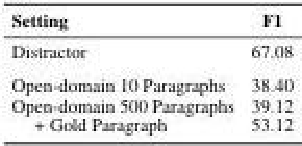
\includegraphics[width=0.3\textwidth]{tmpx9v9v4oi_origin.pdf}\\
    \hline
    \textbf{Question} & By how much does the F1 score improve when the gold paragraph is added to the open-domain setting with 500 paragraphs? \\
    \hline
    \textbf{Answer} & The F1 score improves by 14.00 when the gold paragraph is added.\\
    \hline
    \textbf{RAG-Anything} & 
    \textbf{F1 Score Improvement Overview}\newline
    Based on the information available, there are various numerical values provided in the context. The relevant values that seem to relate to performance measurements, possibly including the F1 score, are 38.40, 39.12, 53.12, and 67.08. These numbers might represent metrics used in evaluating an open-domain text composition task, such as the ones mentioned regarding different paragraph settings [KG] Open-domain 10 Paragraphs - Open-domain 500 Paragraphs + Gold Paragraph.\newline
    Although the exact nature of the improvement in F1 score is not explicitly stated, we can infer from the context provided that an enhancement might be associated with the addition of the 'Gold Paragraph' in the open-domain settings involving 500 paragraphs. The exact degree of improvement, however, would require detailed data that is not present in the provided context.\newline
    \textbf{Conclusion}\newline
    It is not possible to definitively determine by how much the F1 score improves when the gold paragraph is added based on the information available as it lacks specific comparative details directly related to the F1 score.\newline
    \textbf{References}\newline
    - [KG] Open-domain 10 Paragraphs - Open-domain 500 Paragraphs + Gold Paragraph\newline
    - [KG] 38.40 - 53.12\newline
    - [KG] 39.12 - 67.08\newline
    - [DC] tmpx9v9v4oi.png \\ \hline
    \end{tabular}
    }
    \vspace{-0.2in}
  \end{table}


\bibliographystyle{unsrt}
\bibliography{references}

\end{document}
